%%%%%%%%%%%%%%%%%%%%%%%%%%%%%%%%%%%%
% This is the template for submission to ISCA 2018
% The cls file is a modified from  'sig-alternate.cls'
%%%%%%%%%%%%%%%%%%%%%%%%%%%%%%%%%%%%

\documentclass{sig-alternate} 
\usepackage{mathptmx} % This is Times font

\newcommand{\ignore}[1]{}
\usepackage{fancyhdr}
\usepackage[normalem]{ulem}
\usepackage[hyphens]{url}
\usepackage{microtype}
\usepackage{fixltx2e}
\usepackage{array}
\usepackage{multirow}

% Always include hyperref last
\usepackage[bookmarks=true,breaklinks=true,letterpaper=true,colorlinks,linkcolor=black,citecolor=blue,urlcolor=black]{hyperref}

% Ensure letter paper
\pdfpagewidth=8.5in
\pdfpageheight=11in


%%%%%%%%%%%---SETME-----%%%%%%%%%%%%%
\newcommand{\iscasubmissionnumber}{NaN}
%%%%%%%%%%%%%%%%%%%%%%%%%%%%%%%%%%%%

\fancypagestyle{firstpage}{
  \fancyhf{}
\renewcommand{\headrulewidth}{0pt}
  \fancyhead[C]{\normalsize{}} 
  \fancyfoot[C]{\thepage}
}  

\pagenumbering{arabic}

%%%%%%%%%%%---SETME-----%%%%%%%%%%%%%
\title{NATCH: A Neural Networks Based Thottler for Hardware Prefetching} 
\author{}
%%%%%%%%%%%%%%%%%%%%%%%%%%%%%%%%%%%%

\begin{document}
\maketitle
\thispagestyle{firstpage}
\pagestyle{plain}

\begin{abstract}
Hardware prefetching has been introduced in modern processors as a way to hide
cache latencies.  An efficient prefetcher should be able to identify complex
memory access patterns during program execution. This ability enables the
prefetcher to read a block ahead of its demand access, potentially saving a
cache miss. Accurately identifying the right blocks to prefetch is essential
to achieving high performance from the prefetcher.

In this paper, we introduce Perceptron-based Prefetch Filtering to help make
this prefetching decision accurately. The perceptron layer acts as a check 
to filter out the unnecessary prefetches recommended by the underlying
prefetcher.  We have also explored a range of features that can be used to
train the perceptron layer.  Our results show that perceptron-based filtering
improves performance on the memory intensive subset of the SPEC 2017 benchmark
suite by 6.84\% on single-core and by 11.9\% on multi-core traces, as compared
to a state-of-the art prefetcher.  We also demonstrate that the performance
gained from using our efficient filter scales better with increasing numbers
of cores.

\end{abstract}

\section{Introduction}
\label{Introduction}

Processor and memory technologies have been developed with different
goals in mind. While processor scaling has focused on speed
improvements, memory scaling has primarily focused on increasing
capacity. The difference in each technology's scaling has led to the
Memory Wall~\cite{MemWall} -- the increasing gap between processor and
memory performance. Data prefetching is one important technique that
has been developed to minimize the effects of this trend.

%Data prefetching exploits the fact that in most applications,
% memory accesses have a repeating and predictable pattern to speculatively fetch useful data from slower levels
%of the cache hierarchy into faster higher levels of cache. %phrasing?

An ideal prefetching scheme would perfectly capture a program's memory
access pattern, and then predict and pre-load the needed data into the
processor's caches in a timely manner.  Memory access patterns may be
simple, such as accessing every item in an array with a for-loop, or
very complex, such as chasing pointers through dynamically-allocated
memory.  % Practical prefetchers face challenges not only in predicting
% what data will be useful in the future, but also in timing when data
% should be prefetched, deciding which level of the cache hierarchy the
% data should be stored in, and deciding what data should be evicted
% from the caches to accommodate the prefetched data.
All prefetchers are designed around a fundamental trade-off between
two important metrics: coverage and accuracy. Prefetcher coverage
refers to the fraction of baseline cache misses that the prefetcher
pulls into the cache prior to their reference.  For example, if an
application experiences 1,000 cache misses without a prefetcher, while
800 of those cache misses become hits with a prefetcher, then the
prefetcher has 80\% coverage for that application.  Prefetcher
accuracy refers to the fraction of prefetched cache lines that end up
being used by the application. So if a prefetcher prefetches 1,200
cache lines, but only 800 of them are used by the application, then
that prefetcher's accuracy is 66.7\%.


\begin{figure}[t]
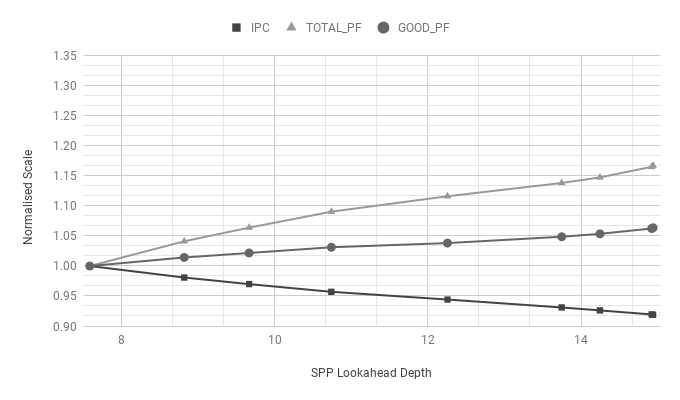
\includegraphics[width=\columnwidth]{Motivation}
\caption{The impact of aggressive prefetching on performance for {\tt 603.bwaves\_s}. 
The number of useful prefetches increases with aggressiveness
slower than total prefetches, which wastes bandwidth and 
harms performance.}
\label{Fig:Motivation}
\end{figure}

Coverage and accuracy are generally at odds with one another, and as
one metric improves, the other usually gets worse. For example, when
an application accesses a new region of memory for the first time, a
na\"ive prefetcher may predict that all data in that region will be
used by the application.  This will clearly result in 100\% coverage
for that region, but with possibly a very low accuracy.  In fact, so
much cache capacity and bandwidth may be wasted prefetching unused
data that performance can ultimately be harmed by this strategy. At
the other extreme, another prefetcher may be overly conservative and
never prefetch anything, wasting no capacity or bandwidth, and
achieving 0\% prefetch coverage.

Figure~\ref{Fig:Motivation} illustrates the above scenario.  Here we
consider a state-of-the-art lookahead prefetcher -- SPP~\cite{SPP}.
Lookahead prefetchers such as SPP provide a mechanism to speculate an
arbitrary number of references ahead of the initial triggering miss.
In SPP, a throttling confidence threshold is then used to ensure that
the lookahead stops when confidence falls too low to ensure that
prefetches are accurate.  In the figure, we iteratively re-tuned 
this threshold to allow the prefetcher to lookahead a fixed
depth from 7 to 15. The figure depicts the behavior 
of the {\tt 603.bwaves\_s} SPEC CPU 2017 benchmark. The IPC, the 
total number of prefetches issued by the prefetcher (TOTAL\_PF), 
and the actual useful predictions (GOOD\_PF), all have been normalized 
to lookahead depth 7. As the lookahead
depth increases, so do useful prefetches, and hence coverage. This
coverage, however, comes at the cost of total prefetches increasing at
an even higher rate. This leads to cache pollution and bandwidth
contention, and leads to a reduction in IPC.  
%Similar behavior was observed in 12 other SPEC CPU 2017 benchmarks.

Therefore, a delicate balance between coverage and accuracy is
required for a prefetcher to maximize its performance impact.
Prefetchers are generally designed with internal mechanisms to monitor
their accuracy, and throttling mechanisms that can be tuned for either
coverage or accuracy.  The more irregular an application's memory
access pattern is, the more difficult it is to accurately predict
every access, so a prefetcher will have to be tuned more toward
coverage (and away from accuracy) in order to gain any benefit. This
may be especially dangerous to do in the context of a multi-core
processor, where overly aggressive prefetching in one core can waste
shared resources, such as last-level cache (LLC) capacity, and
off-chip bandwidth, impacting the performance of other
cores~\cite{Friendly}.

% Predicting future accesses requires a trade-off between coverage,
% the percent of predictions that prevented a cache miss, and
% accuracy, the percent of predictions made that were correct.
%% Gino: Just added a short explanation of coverage and accuracy
%% tradeoff, not sure if necessary
%A prefetcher may have high coverage by reducing the number of misses
% by simply requesting a large amount of data, however this does not
% imply accuracy. Even if the prefetcher brought in data accessed in
% the future, a high percentage of the data requested could never be
% accessed meaning the prefetcher had low accuracy, resulting in
% wasted resources as well as cache pollution. Likewise, a prefetcher
% can have a higher accuracy by being completely sure the data
% requested is used in the future, but may not affect performance
% since it did not have the coverage needed to make an
% impact. %end addition.
% Most prefetchers maintain an internal confidence mechanism by
% keeping counters to track events such as cache hits, misses,
% references to an entry in the prefetcher's structure, etc. By
% comparing the confidence indicated by the counters against different
% threshold values, the aggressiveness of the prefetcher can be
% adjusted, resulting in lower coverage and higher accuracy.

%For a prefetcher to capture highly irregular access patterns, it
% needs to be highly aggressive with high coverage. This causes the
% prefetcher to recommend many low accuracy prefetches that lead to
% the cache being polluted with useless data.  This effect is more
% pronounced in a multi-core scenario where the LLC is a shared
% resource~\cite{Friendly}. Conversely, a conservative prefetcher
% would be highly accurate but might not make enough useful prefetches
% due to its lower coverage.

Here, we propose Perceptron-based Prefetch Filtering (PPF) as an
enhancement to existing state-of-the-art prefetchers, allowing them to
speculate deeply to achieve high coverage while filtering out the
inaccurate prefetches this deep speculation implies.  PPF works by
observing the stream of candidate prefetches generated by a
prefetcher, and then rejects those that are predicted by the
online-trained neural model to be inaccurate.  The state-of-the-art
prefetcher that we use to evaluate PPF in this paper is the Signature
Path Prefetcher (SPP)~\cite{SPP}, however as we describe, PPF can be
designed to benefit any prefetcher.  In this design, PPF replaces
SPP's existing confidence-based throttling mechanism, which itself was
a highly tuned feature of that prefetcher.  Because PPF is so much
more effective at rejecting inaccurate prefetches than SPP's 
{\color{red}internal} mechanism, we are free to re-tune the rest of 
SPP's design around maximizing coverage. The result is an increase 
in both accuracy and coverage, and a notable increase in performance.

%We propose Perceptron-based Prefetch Filtering (PPF) as an enhancement to
%the existing state of the art prefetchers to robustly overcome the coverage
%vs. accuracy trade-off. The idea is to use a state-of-the-art prefetcher as
%the base engine. For that we choose Signature Path Prefetcher (SPP) and
%modify the design to make it as aggressive as possible. This modification
%enables the base engine to capture complex memory access patterns and go
%deeper into the speculation path, increasing coverage without sacrificing accuracy. 
%Normally such aggressive prefetching would come at the cost of increased DRAM traffic
%and cache pollution. However, prefetch suggestions recommended by the base prefetch
%engine are passed through the perceptron based filter to ensure an accurate prediction.
%Over time, PPF learns to correlate the prefetch recommendations with various available
%features, leading to elimination of useless prefetches. This filtering leads
%to overall increased accuracy of the prefetch scheme and reduction in DRAM
%traffic and cache pollution.

This paper describes PPF, explains its merits, offers analysis, and
outlines the scope for future research. Its contributions are:

\begin{itemize}

\item An on-line neural model used for hardware data prefetching.
  Previous work in this area either relied on program
  semantics~\cite{Semantics} or were application
  specific~\cite{Datacenter}.

\item Implementing PPF filtering a state-of-the-art prefetcher, giving
  a significant performance improvement compared to previous work. PPF
  learns to adapt itself to shared resource constraints, leading to
  further increased performance in multi-core and
  bandwidth-constrained environments.

\item A methodology for determining an appropriate set of features for
  prediction, regardless of the underlying prefetcher used.  More
  details are explained in Section \ref{Method-Features}.

\end{itemize}

In a single core configuration, PPF increases performance by 3.78\%
compared to the underlying prefetcher, SPP. In a multi-core system running a
mixes of memory intensive SPEC CPU 2017 traces, PPF saw an improvement
of 11.4\% over SPP for a 4-core system, and 9.65\% for an 8-core system.

% djimenez - cutting this
%The paper is organized as follows. Section~\ref{Background} describes
%background work and summarizes SPP. Section~\ref{Arch} gives the 
%architectural overview of PPF. Section~\ref{Impl} discusses the
%implementation of PPF using SPP and the particular features used.
%Section~\ref{Method} gives the evaluation methodology and explores the feature
%space for perceptron learning. Section~\ref{Results} evaluates the
%performance of the prefetcher and Section~\ref{Conclusion} concludes the
%paper.

\section{Background Work and Motivation}
\label{Background}

In this section, we compare the existing work done in the domain of
prefetching.  We also discuss about some of the interesting memory
access patterns seen in the workloads in SPEC 2017 benchmark.  The
second half of this section deals with a background of Signature Path
Prefetcher architecture.

\subsection{Related Work}
\label{Background-Related}
The idea of prefetching has been around since Instruction Stream
Buffers were proposed by Jouppi~\cite{ISB}. Some of the earliest data
prefetchers developed to try to identify memory access patterns with a
constant stride pattern~\cite{Smith,Baer,Stride}. Major research was
dedicated to stride distance and depth prediction~\cite{Decoupled,Adaptive}. Newer prefetchers aimed at correlating
predictions with the past memory access addresses~\cite{Address_Correlated,AMPM}.

With time newer and more intricate prefetchers were
introduced~\cite{Wenisch_Temporal_Streaming,Stealth,Feedback_Directed,Coordinated,Bandwidth_Efficient,Pacman,TLB,Linearizing,Sandbox,VLDP,DoL,Domino}.
A whole class of streaming prefetchers developed on the lines of
Spatial / Temporal Memory
Streaming~\cite{Spatial_Pattern,SMS,Temporal_Instruction_Fetch,Off_Chip,STMS,SMS_JILP}.
There have been ideas for control flow speculation directed hardware prefetching~\cite{BFetch,MTBFetch}.

Most modern prefetchers aim at identifying complex memory access
patterns in a given application.  This allows them to capture some of
the irregular patterns seen in pointer chasing data-structures.
Offset based prefetchers are a generalization of the next-line
prefetcher.  Some of the prominent prefetchers exploiting this idea
are Sandbox Prefetcher~\cite{Sandbox} and the Best Offset Prefetcher~\cite{BOP}. 
Another class of prefetchers is lookahead Prefetchers.
Such prefetchers try to speculate deep into the application's memory
access trail.  These include Path Confidence based Lookahead
Prefetching~\cite{SPP} and Kill the Program Counter~\cite{KPC}.

A related line of work also explores cache replacement - insertion
policies and dead block prediction, with an eye towards
prefetching~\cite{DB_Pred,Cache_Burst,KPC,Harmony}.  Nori
\textit{et.al.} introduced prefetching with respect to runtime
criticality~\cite{CATCH}.

\textit{Machine Learning and Prefetching:} Peled \textit{et.al.}
introduce interesting ideas for on-line Reinforcement Learning and
dynamically scaling the magnitude of feedback given to the baseline
prefetcher~\cite{Semantics}. The biggest challenge here is that it
relies on compiler support for getting features to build the context.

The paper by Liao \textit{et. al.} focuses on prefetching for data
center applications~\cite{Datacenter}. They use offline Machine
Learning Algorithms like SVMs and Logistic Regressions to do
parametric search for an optimal prefetcher configuration.

%% NOTE: The below paper is literally the same idea as ours. But poor implementation and no good results. How much to bash this paper?
Finally, the paper on Data Cache Prefetching with Perceptron
Learning~\cite{BadPerc} talks about the idea of two step prefetching.
The first step is an existing baseline prefetcher while the second
step is a perceptron based throttler.  The paper has lots of
limitations in terms of design and implementation.  That reflects in
the fact that it did not lead to any significant performance gain over
even the basic prefetchers like the Stride Prefetcher~\cite{Stride} and
the Markov Prefetcher~\cite{Markov}.


\subsection{Perceptron Learning in Architecture}
\label{Background-Perceptron}
Perceptron learning for computer architecture design has been around
for a while.  It was first popularized by Jimenez \textit{et. al.} for
doing branch prediction~\cite{Perc_Branch}. In it's original
implementation, the Program Counter of the instruction looking for a
branch prediction would index into a given table of perceptron
weights.  The retrieved weights would then be multiplied with the
history of branch outcomes stored in the History Register (which is a
feature) in a dot product fashion.  The sum obtained is thresholded at
0 \textit{i.e.}, if the prediction y\textsubscript{out} >= 0, the
prediction is made as \textit{true}, or branch taken.  Else if the sum
is < 0, the prediction is made as \textit{false}.

The structure that we use is derived from the model introduced in
Piecewise Linear Branch Prediction~\cite{Piece_Linear}.  Here the
feature itself is used to index into a hash of perceptron weights.
This form of indexing makes sure that the hyper-plane learned by the
perceptron weights is able to differentiate between linearly
inseparable outcomes.  \textit{<Is it true? Not sure>}

Perceptron Learning for Reuse Prediction~\cite{Perc_Reuse} extended the
hash perceptron architecture to perform prediction in context of cache
replacement.  Perceptron layer can learn to correlate the cache
replacement behaviour with a variety of features.  Each feature has
its dedicated table of perceptron weights which it indexes into.
Hence number of tables equals the number of features.  Once the
perceptron weights from all the tables are obtained, they're summed
and thresholded based on a pre-decided value.  This led to a
prediction mechanism that is highly accurate, has quick learning rate
and is adaptable to changing program behaviour.  The features
introduced in that paper were derived from Program Counters of the
current and the last few instructions and from the memory address of the
current access.  Even with such basic features, high level of
correlation could be established by perceptrons.

The work was further extended by Multiperspective Reuse
Prediction~\cite{Multiperspective}, which introduced a varied set of
parametric features.  Although design space exploration for feature
and parameter selection was a non-trivial task, once fixed, it could
give a cache replacement predictor highly suitable for the given set
of applications.

\textit{Deviations From Actual Perceptrons:} Traditionally, a
perceptron prediction involves multiplying the vector of input
features: F\textsubscript{1xN}, with the corresponding weight vector:
W\textsubscript{Nx1} in a dot product fashion to obtain the sum
y\textsubscript{out}.  Here what we use is a perceptron-like
structure.  The feature is used to hash into the weight of perceptrons
and the retrieved weights are added straight away.  This can be seen a
dot product of $\vec{1}$\textsubscript{1xN} with W\textsubscript{Nx1}.
This way, the perceptron algorithm doesn't introduce any
multiplication operations in the inference or training process.  Hence
what we adapt in this work, is a perceptron-like learning algorithm as
it involves the same principle involved in perceptron inferencing and
training.  For simplicity, we will call our implementation as
perceptron implementation.

\textit{Perceptron Update Rule:} In all the above implementations, a
uniform perceptron update principle is being followed.  The weights
need to be updated if the prediction was wrong or the predicted sum
does not cross a certain threshold.  After a certain training period,
these weights are proportional to the probability of the outcome being
true.  This training threshold makes sure that the perceptrons are
trained till a certain level of confidence and yet they are not
over-trained to the given set.  Care is taken that the weights
saturate at certain positive and negative values so that they remain
confined to the bit-width.  The same rules will be applied in the
discussion done in Section \ref{Design-Perceptron} on NATCH learning algorithm.

 
\subsection{Prefetching with SPEC 2017}
\label{Background-SPEC2017}
\textit{<Discuss SPEC 2017 traces here>
<What are the possible graphs / analysis tools we can use for SPEC traces?>}

\subsection{Signature Path Prefetcher Architecture}
\label{Background-SPP}
Since the work we have done uses SPP~\cite{SPP} as the underlying prefetcher, we are
presenting a brief recap of the ideas introduced in the original
paper, especially with an eye towards their relevance in our work.
Signature Path Prefetcher (SPP) is a lookahead prefetcher and consists
of following structural components:

\textbf{Signature Table:} The ST keeps track of 256 most recently accessed
pages.  It is meant to capture memory access patterns within a page
boundary.  SPP indexes into an entry of ST using the page number.  For
each entry corresponding to a page, ST stores the `last block offset'
and `old signature'.  Last block offset is the block offset of the
last memory access of that given page.  The block offset is calculated
with respect to the page boundary.  The signature is a 12-bit
compressed representation of the past few memory accesses for that
page.  The signature is calculated as:
$$New Signature = (\,Old Signature << 3 bits\,) \;\;XOR\;\; (\,Delta\,)$$ 
In case a matching page entry is found, the stored signature in the corresponding entry is retrieved.

%% NOTE: Can we do away with this example? 
%%       If it looks like we are weiting too much about SPP
Consider the case that incoming page number 10 with a block offset 3
finds a match in the ST.  The retrieved pattern signature is 0x30 and
the Last Offset is 1.  Since now there is the Last Block Offset (1),
Incoming Block Offset (3), Old Signature (0x30), and New Signature
calculated as per above equation (0x182), SPP can infer
non-speculatively that the given pattern of memory accesses (as
captured in the Old Signature) leads to the particular Delta.  In
general, Delta is defined as the difference between the prefetch
suggestion block and the initial block which triggered the prefetch.
In this case, since SPP is in learning phase, it is defined as the
difference between the Incoming Block Offset and the Last Block Offset
(+2 in this case).  This, in turn generates the new memory pattern
(New Signature).  This newly learned signature pattern and the delta
is stored in the Pattern Table.

\textbf{Pattern Table:} The PT is indexed by the signature generated
from ST.  PT holds predicted delta patterns and their confidence
estimates.  Each entry indexed by the signature holds up to 4 unique
delta predictions.  This is implemented by making PT as a 4-way
associative table.  To measure an estimate of a delta confidence, PT
implements two counters: C\textsubscript{sig} for each entry indexed
by the signature and C\textsubscript{delta} for each delta entry for a
given signature.  More details of this on-line score-keeping mechanism
is described under Confidence Tracking discussion.

\textit{Lookahead Prefetching:} On each trigger, SPP tries to go down
the program speculation path using its own prefetch suggestion.
Using current prefetch as the baseline, it re-accesses the PT to generate further
prefetches.  It keeps on repeating this cycle of accessing PT and
updating the signature based on highest confidence prefetch from the
last iteration.  These iteration count till which SPP manages to
predict prefetch entries in the lookahead manner is characterized as
its `depth'.  While doing this, SPP also keeps compounding the
confidence in each depth.  Thus as depth increases, overall confidence
keeps decreasing.  

\textbf{Global History Register:} The GHR is a small 8-entry fully
associative structure to bootstrap learning across page boundaries. 
Whenever a prefetch suggestion from the
Pattern Table crosses page boundaries, instead of completely
discarding it, GHR saves that information for inter-page learning.
Since our NATCH implementation in this paper doesn't affect GHR
functionality in any ways, we won't be going into more details about
GHR.

\textbf{Prefetch Filter:} SPP also introduced the concept of Prefetch
Filter - a 1024 entry 1-way associative table which keeps a record of
last few entries prefetched.  This proves useful for following
reasons:
\begin{itemize}
\item \textbf{Eliminating duplicate prefetches}\newline Any subsequent
  prefetches recommended by SPP mechanism are checked against the
  existing entries in Prefetch Filter.  If a valid entry is found, it
  means that the particular cache line is already either in L2 Cache
  or being fetched.  Hence there is no need to issue a duplicate
  prefetch.
    
\item \textbf{Updating prefetcher}\newline Since the PF keeps a track
of past few prefetches, it uses that information to see if a given
prefetch led to a demand hit or a cache eviction. Using this information, 
SPP can update its internal states.
    
\item \textbf{Tracking Global Accuracy}\newline PF keeps a track of
  global usefulness ($\alpha$) of the prefetches by calculating 
  C\textsubscript{useful} / C\textsubscript{total}, where
  C\textsubscript{total} is the total number of prefetches
  getting recorded in the PF and C\textsubscript{useful} is the number 
  of prefetches that led to a demand hit.
\end{itemize}

\textbf{Confidence Tracking}: The PT keeps a track of hits to each
signature through a counter C\textsubscript{sig}.  The number of hits
for a given delta per signature are tracked using a counter
C\textsubscript{delta}.  The confidence for a given delta is
approximated through C\textsubscript{d} = C\textsubscript{delta} /
C\textsubscript{sig}.  When SPP enters into a lookahead mode, the path
confidence P\textsubscript{d} is given as:
$$P\textsubscript{d} \;=\; \alpha  \;.\;  C\textsubscript{d}  \;.\;  P\textsubscript{d-1}$$ where $\alpha$ is called the global accuracy and is calculated as shown previously. 
The range of global accuracy ($\alpha$) is [0,1].

Here d is the lookahead depth.  For d = 1, when SPP is in
non-speculative mode, P\textsubscript{0} can be thought of as 1. 
The final P\textsubscript{d} is thresholded against prefetching-threshold
(T\textsubscript{p}) to decide whether to prefetch or not.  If yes,
then P\textsubscript{d} is thresholded against a numerically bigger
fill-threshold (T\textsubscript{f}) to decide whether the prefetch
should be sent to L2 Cache (high confidence prefetch) or Last Level
Cache (low confidence prefetch)

<Insert a comprehensive figure about SPP structures>

<Insert another detailed picture about SPP data-path flow>

\subsection{Case for an On-line Throttler}
\label{Background-Case}
As compared to some of the other state of the art prefetchers [BOP],
SPP is a less aggressive prefetcher.  In the single core
environment, this gives BOP an edge as there is no resource contention
among the different cores.  Hence more aggressive prefetching is bound
to prove beneficial.  As we increase the core count, we observe that
SPP starts outperforming rest of the prefetchers.  This can be
attributed to the fact that each prefetch suggested by SPP is a
carefully calculated one and that prevents cache pollution.
\textit{<Figure showing the variation of SPP vs BOP wrt core count>}
For 4-core applications, SPP suggests XX\% fewer prefetches than BOP
and yet leads to higher IPC.

The above analysis shows that with a more careful throttling
mechanism, any prefetcher like SPP can be tuned to become much more aggressive, leading to
increased coverage.  The onus of maintaining the accuracy now falls on
the independent throttler.  To test the hypothesis, we tuned down SPP
to the minimum possible threshold.  Only by doing this we managed to
increase the prefetch suggestions made by SPP, by XX\%.
\textit{<Comparison of SPP-Unleased with SPP / BOP>} Obviously this
came at a cost of increased DRAM traffic and cache pollution.

Moreover, the on-line confidence mechanism introduced in SPP was very
rudimentary.  It was based on taking a ratio C\textsubscript{d} =
C\textsubscript{delta} / C\textsubscript{sig} as explained above.  The
same confidence was used to make the decision whether to prefetch or
not to prefetch; and which level to prefetch.  While this
approximation was shown to work in the original implementation, we believe that a
better form of generalised on-line decision making was possible.  
Hence, it was
necessary to build a robust and adaptable learning mechanism to accept
/ reject the prefetch suggestions; and to decide the fill level (L2
Cache vs Last Level Cache).

To that effect, we introduce an independent on-line perceptron based throttling mechanism.

\section{PPF Architecture}
\label{Design}

In this section we describe our implementation of PPF.  PPF is a generalised
prefetch throttler and can be adapted to most prefetchers with minimal
modifications.  For a practical implementation, we have used SPP as the base
engine prefetcher.

\subsection{Changes made to original SPP}
\label{Design-Changes}
To modify the SPP design to suit our scheme, the following changes were made:

\begin{itemize}
\item \textbf{Original Thresholds discarded}\newline In the original
  SPP design, the internal confidence was compared against a preset
  PF\_THRESHOLD (T\textsubscript{p}) to decide whether to accept or reject the
  prefetch suggestion.  Furthermore, the accepted suggestions were thresholded
  against FILL \_THRESHOLD (T\textsubscript{f}) to decide the fill level: L2
  Cache vs Last Level Cache.  T\textsubscript{p} and T\textsubscript{f} were
  set to 25 and 90 respectively, on the scale of 0 to 100.  In PPF, the
  perceptron sum is used to make these decisions.  Hence these two thresholds
  are no longer needed

%%[NOTE] Can this point be removed?
% djimenez: I think this would be necessary to reproduce our results so leave it in. 

\item \textbf{Looking at L2 MSHR Queue while prefetching}\newline The original
SPP would not consider the slots available in the L2 MSHR queue.  It had an
assumption that at no time can the number of prefetches suggested by SPP
exceed the capacity of the queue.  While it was not proven in the paper, the
internal confidence mechanism along with the thresholds made sure that the
above assumption was maintained.  In PPF since there can be no assumption on
the degree of aggressiveness of the underlying prefetcher, we explicitly check
that at no point should the number of suggested prefetches exceed the L2 MSHR
queue.

\item \textbf{Enhanced Filter}\newline The original SPP introduces a concept of
the Prefetch Filter that keeps a track of up to 1024 L2 cache prefetch
suggestions.  For PPF, the Filter was modified to store metadata such as program
counter, memory access address etc.  These features are needed to train the perceptron
when the result of that particular prefetch becomes available.  At training time,
this data is used to retrieve the state of the prefetcher when the prediction
was made.

\item \textbf{Reject Filter introduced}\newline The Prefetch Filter mentioned
above keeps track of the prefetches that actually happened in the L2 Cache.
Correspondingly, we introduced a reject filter.  It keeps track of the
prefetches that were suggested by the base SPP engine but were rejected by the
perceptron.  In case it is detected that a future demand fetch could have used
this rejected prefetch, the perceptron weights are updated to reflect that
misprediction.

\end{itemize}

\subsection{The Perceptron Layer}
\label{Design-Perceptron}
As discussed earlier, the perceptron layer was introduced to act as a
throttler to the underlying prefetch engine.  This section explores the
details of the perceptron layer and the range of features that are ultimately
used by the perceptron for correlating the prefetches.

The weights are stored in separate tables for each
feature.  Features are indexed using different numbers
of bits.  At most 12 bits of a feature are used to index into a
weights table.  Certain features require more resolution power
\textit{i.e.}, the full 12 bits of indexing.  On the other hand, some
features requiring lower resolution require as few as 7 bits of
indexing.  The variable indexing was determined by studying the
features and fine-tuned empirically so as to achieve a good accuracy
vs area trade-off.  Exact details are mentioned under ``Area Overheads''
in Section~\ref{Method-Overheads}

A single entry in the table corresponds to a perceptron weight.  Each
weight is a 5 bit counter - saturating at -16 and +15.  Each feature
has its own dedicated table.  Our proposed design uses 9 features.
As program execution begins, all the weights are initialized to 0.

\textbf{Inference}\newline In the ChampSim simulator, the prefetching method
is triggered on every L2 Cache demand access.  At that point, the prefetcher
has the option to do or not do a prefetch -- if it does, then it has a choice
in how many cache lines to prefetch.  The suggested prefetches can be either
in the L2 Cache or the last-level cache.  The prefetcher decides this
placement, and it is usually done based on an internal confidence mechanism.

When the base prefetcher is triggered, it starts suggesting candidates for
prefetching.  All these recommended prefetches are tested in the perceptron
throttler before they can access the Prefetch Filter, as in the original SPP
datapath.

The perceptron looks at the microarchitectural state, {\em i.e.} the features,
at that instant.  Each feature is hashed to form an index into a table of up to 
4096 entries dedicated for that feature.  
Feature \#1 indexes into
a particular entry in table \#1 and so on.

Once all the weights are retrieved, they are summed.  The sum is thresholded
based on the preset threshold PERC\_THRESHOLD\_LO.  Only the prefetch
candidates with perceptron sum higher that the threshold qualify for
prefetching.  The prefetches that qualify through the perceptron throttler
stage go through the Prefetch Filter stage.  The Prefetch Filter eliminates
any redundant prefetch suggestions.  In PPF, all the metadata that is required
to recreate the features is also stored in the Prefetch Filter.  At a later
stage, when the feedback of the current prefetched line is available, the
stored data is used to train the perceptron.

The perceptron sum is also used to decide L2 Cache vs Last Level Cache
placement of the prefetch cache line.  All prefetch candidates qualified till
this stage are thresholded against PERC\_THRESHOLD\_HI to decide the fill
level. The two thresholds: PERC\_THRESHOLD\_LO and PERC \_THRESHOLD\_HI are
empirically set.

The perceptron sum can also be seen as the sum of the individual contribution
per feature.  The value of each contribution corresponds to the extent of
confidence of the final output with that given feature.  By summing the
individual contributions, the final perceptron sum denotes the overall
confidence for that prefetch suggestion.  By thresholding the perceptron sum
on two different thresholds, we are dividing the confidence scale of the
prefetch suggestion into three bins.  The first bin corresponds to the lowest
confidence leads to prefetch candidate being rejected.  The next bin
corresponds to prefetches with a moderate confidence level.  Such prefetches
are directed to fill the bigger Last Level Cache and potentially not pollute
the more scarce L2 Cache.  The highest confidence prefetches are filled in the
L2 Cache.

In addition to the Prefetch Filter mentioned above, PPF also maintains a
``Reject Filter.''  The reject filter is a 1024-entry deep direct-mapped
table.  If a prefetch suggestion is rejected by perceptron throttler, it is
logged into the Reject Filter.  The filer is used to train the perceptron to
avoid false negatives \textit{i.e.}, cases where prediction was to reject the
prefetch but the prefetch would have been useful.

% djimenez: if it were previously stated then it's redundant here? do we need
% this statement?

%As previously stated all the metadata describing the program state at the
%instant of prefetching is stored in the Prefetch Filter or the Reject Filter.
%This information is useful when the perceptron needs to be updated
%subsequently.

\textbf{Training}\newline In the prefetching environment, feedback for a
prefetch is received whenever there is an eviction or a demand access from the
L2 Cache.  This action triggers training of the base prefetcher as well as the
perceptron throttler.  Training the perceptron throttler involves restoring
the metadata that was stored in Prefetch Filter or the Reject Filter.  This is
done by indexing into the corresponding filters using the cache line address
of the block being used to train. (10-bits indexing + 6-bits tag matching).
Once the state of the program at the time of prefetching is available, it is
used to index into the perceptron weights table.

If a demand access block that triggers the training was tagged as a valid
prefetch in the Prefetch Filter, then the earlier prefetch prediction was
correct.  In that case the perceptron weights are incremented by 1 if the
predicted sum does not cross a pre-defined threshold.  If a cache block
eviction led to training and the corresponding valid entry was found in the
Prefetch Filter, then the prediction made by the perceptron was wrong.  The
perceptron should have ideally rejected the prefetch suggestion as a
low-confidence prefetch.  Here the weights are decremented by 1 to reflect the
misprediction. In either case, weights are saturated at -16 or +15.

A secondary training mechanism also kicks in during demand fetches.  Before
the demand access triggers the next set of prefetches, Reject Filter is
checked for a valid entry.  A hit means that the corresponding cache line was
initially suggested by the underlying prefetch engine but rejected by the
perceptron throttler.  Thus, the perceptron should have been more confident
about that particular prefetch.  Once such a scenario is identified, the state
of the execution at the time of prefetch is retrieved from the Reject Table.
The retrieved data is used to index into the various weights tables of the
perceptron and the corresponding values are updated by +1, saturating between
and -16 and +15.  This update reflects increased confidence for the prediction
corresponding to that prefetch.

This mechanism allows us to solve the classical problem of exploiting a lost
opportunity.  In prior perceptron based implementations (and in general,
prefetching algorithms), there is usually no way of knowing the result of not
prefetching a particular line.  Our two-step PPF architecture allows us to
overcome that issue.

\subsection{Features used by Perceptron}
\label{Design-Features}
Here we discuss the various features that correlate the prefetching decision
with the program behaviour.

\begin{itemize}
\item \textbf{Base Address} of the demand access that triggered the
  prefetch.  Since prefetches are triggered from the L2 demand access,
  they tend to be correlated with the triggering address.

\item \textbf{Cache Line} and \textbf{Page Address}: These two
  separate features are derived from the base address that triggered
  the prefetch, as follows: base\_addr >> LOG2\_BLOCK \_SIZE and
  base\_addr >> LOG2\_PAGE\_ SIZE respectively.  The idea behind using
  three different shifted versions of the same feature is that it
  allows us to look into a wider range of bits than with a single
  version.  It also helps give more importance to the overlapping bits
  and lesser importance to most and least significance bits.  This
  approach can also eliminate destructive interference that can be
  caused by directly folding the bits into half.

% djimenez: this is a nice intuition and explanation.

\item \textbf{Program Counter XOR Depth}: The PC is for the instruction
  that triggered the prefetch chain.  Depth refers to the iteration count of
  the lookahead stages.  In general, the PC is not considered as a good basis
  for doing lookahead prefetching as all the prefetches with depth >= 1 are
  aliased into the same PC which would not be true in an actual demand access.
  This feature resolves a PC into a different value for each lookahead depth
  of prefetch speculation, giving a more accurate correlation in lookahead
  cases.  This is akin to the concept of Virtual Program Counters~\cite{VPC}
  introduced by Kim \textit{et. al.} for indirect branch prediction.

\item \textbf{PC\textsubscript{1} XOR PC\textsubscript{2}>>1 XOR
  PC\textsubscript{3}>>2}: Here $PC_i$ refers to the last $i^{th}$
  PC before the instruction that triggered the current prefetch.
  Hashing together the last three PCs tell PPF about the path
  that led to the current demand access and helps capture and
  branching information of the current basic block.  PCs are shifted
  in the increasing order of history before being hashed together.
  This is done to avoid the resultant value of zero in case 2 or more
  PCs are the same.  Additionally, obfuscating the information as it
  gets old allows us to get a wider and an approximate look into the
  program history.

\item \textbf{Program Counter XOR Delta}: This feature tells us if a given PC
  favours particular value(s) of delta.  As noted earlier, while the PC in
  itself does not convey much useful information, this hash resolves the PC
  into different values based on the tendency of that PC to favour a certain
  delta.  Thus, the dynamic nature of different instances of the same memory
  access instruction can be captured here.

\item \textbf{Confidence}: The integer confidence on a scale of 0 to
  100 that was used in the original SPP design.  While the original confidence
  is not used directly for decision making, it can still contribute to the
  final decision made.

% djimenez: this is a little vague. can you be more precise?
\item \textbf{Current Signature XOR Delta}: Recall from
  the discussion of SPP in Section \ref{Background-SPP} that the new signature
  is generated using the old signature and the block delta.  While ``Current
  Signature XOR Delta'' is not the exact formula for generating the future
  signature, it gives an approximate idea of the path that the combination of
  these two values can lead to.

\item \textbf{Page Address XOR Confidence}: This feature scores the tendency
of each page to be prefetch friendly or prefetch averse. It helps resolve a
page into different entries depending on its confidence for prefetching, which
can vary during phases of a program execution.

%%%%%%% Below are the features rejected when downsizing 14 -> 9
% \item \textbf{Current Signature}: The 12-bit signature used by SPP
%   to index into the Pattern Table
% \item \textbf{Delta}: The signed version of the difference in the
%   block address that triggers the prefetch and the block address of
%   the data being prefetched
% \item \textbf{PC}: Program Counter of the Load instruction that
%   triggers that particular prefetch
% \item \textbf{Base address XOR Delta}: If any particular value(s) of
%   delta are highly favoured by a given address which triggered the
%   prefetch, this composite feature can capture that information
% \item \textbf{Cache line XOR Delta}: qThis feature captures if any
%   particular delta is highly favoured by a given cache line address
%\item \textbf{Confidence XOR Delta}: This gives a combined insight
%  into that fact that certain delta-confidence pairqs predicted by
%  SPP might correlate more with the prefetch outcome
%%%%%%%%%%%%%%%%%%%%%%

\end{itemize} 

Some of the composite features are derived from simple hashing (XOR) of two
primary features.  There is always a question of usefulness of such composite
features and the new information added.  We justify the choice of each feature
by quantifying the contribution made towards predicting prefetch behaviour, in
Section \ref{Method-Features}.  Finally, as noted above, each feature indexes
into its independent entry of perceptron weights.

\subsection{Generalizing PPF for any Prefetcher}
\label{Design-Generalizing}
The above implementation of PPF shows that it is highly modular and can be
adapted to be used over any base prefecher for increased prefetch accuracy.
In our implementation, only two hooks are required between PPF and the
baseline SPP. The first is to make sure that all the prefetch candidates of
SPP pass through the perceptron throttler and if qualified, the metadata for
perceptron indexing be stored. The second is needed when the feedback of a
prior prefetch is available in form of a subsequent demand hit or cache
eviction. In that case, the stored metadata needs to be retrieved to update
the state of the perceptrons.

In general, PPF can be adapted to a new base prefetcher with only a few modifications.
\begin{itemize}

\item \textbf{Enhancing the Base Prefetcher:} By tuning down any internal thresholds 
to increase its inherent aggressiveness. 

\item \textbf{Inferencing and Storing:} All prefetch recommendations to be
tested using the perceptron inferencing algorithm.  Perceptron output:
\textit{true} and \textit{false} should be saved appropriately, along with all
the metadata required for perceptron indexing.

\item \textbf{Retrieving and Training:} When the feedback is available, the
previously stored metadata can be used to re-index into the perceptron entries
and increment / decrement the weights.

\item \textbf{Feature Selection:} Six out of the nine features we developed
use information derived from program execution, irrespective of the baseline
SPP prefetcher. Beyond that, the feature set can be expanded to convey any
useful information from the prefetcher to the perceptron throttler.  For
example, in our implementation ``Confidence,'' ``Current Signature XOR Delta,''
and ``Page Address XOR Confidence'' are such features.

\end{itemize}


\section{Methodology}
\label{Method}

\subsection{Performance Model}
\label{Method-Model}
For testing and comparing PPF, we used the ChampSim~\cite{Champsim} simulator.
ChampSim is an enhanced version of the framework that was used for the 2nd
Data Prefetch Championship (DPC-2)~\cite{DPC_2}. We model 1-core, 4-core, and
8-core out-of-order machines. The details of the configuration parameters are
summarized in Table~\ref{tab:Sim_params}.

\begin{table}[]
    \centering
    \begin{tabular}{|l|p{3.6cm}|c|}
    \hline
    Level & Configuration & Access Latency \\
    \hline
         L1 Cache & Separate I-cache and D-cache, 32 KB, 8-way & 4 cycles\\
         L2 Cache & Private, 256 KB & 8 cycles\\
         LLC & Shared, 2MB / core, 16-way & 20 cycles\\
         DRAM & 4 GB Single Channel for single-core, 8 GB Double Channel for multi-core & N?? cycles\\
    \hline
    \end{tabular}
    \caption{Memory Model Parameters}
    \label{tab:Sim_params}
\end{table}

% djimenez: changing all the "was" to "is." when describing our work, use
% present tense

The block size is fixed at 64 bytes. Prefetching is only triggered at an L2 cache
demand accesses but could be directed to the L2 or last-level cache. No L1
data level prefetching is done. The LRU replacement policy is used on all levels
of cache hierarchies. Branch prediction is done using the perceptron branch
predictor~\cite{Perc_Branch}.  ThE page size is 4KB.  Champsim operates
all the prefetchers strictly in the physical address space.

\subsection{Testing Under Additional Memory Constraints}
\label{Method-AdditionalMem}
The default single-core configuration simulates a 2MB LLC and a single
channel DRAM with 12.8GB/s bandwidth.  We extend the simulations to
include memory constraints introduced in DPC-2.  Specifically we look
at the following two variations:
\begin{itemize}
\item \textit{Low Bandwidth DRAM}: Here the DRAM bandwidth is limited
  to 3.2 GB/s
\item \textit{Small LLC}: In this scenario, LLC size is reduced to 512
  KB
\end{itemize}
All the multi-core simulations are only done in the default
configuration.

\subsection{Workloads}
\label{Method-Workloads}
% djimenez: don't say this is the first time SPEC 2017 has been used this way.
% i don't know if that's true, and in any event the value is small.

%This is the first time that SPEC 2017 benchmark suite~\cite{SPEC2017}
%has been used to characterize and measure the prefetch performance.
We use the that SPEC 2017 benchmark suite~\cite{SPEC2017}.  We use all the 20
workloads available in the SPEC 2017 suite.  Using the SimPoint~\cite{SimPoint}
methodology, we identified 95 different program segments of 1 Billion
instructions each.

\textit{Single-core performance:} For single-core simulations, we use 200
million instructions to warm-up the microarchitectural structures and the next
one billion instructions to do detailed simulations and collect run-time
statistics. We report the IPC speedup over the baseline of no prefetching.
The final number reported is the geometric mean of the speedup achieved on
individual traces.

\textit{Multi-core performance:} For multi-application workloads, we generate
100 random mixes and another 100 mixes from the memory intensive subset of
SPEC 2017.  For 4-core workload, 200 Million instructions are used for warm-up
and additional 1 Billion instruction simulated for collecting statistics.
Each CPU keeps executing its workload till the last CPU completes one billion
instructions after warm-up.  For collecting IPC and other data, only the first
billion instructions are considered as the region of interest.

Here we report the weighted speedup normalized to baseline
\textit{i.e.}, no prefetching.  For each of the workloads running on a
particular core of the 4-core 8 MB LLC system, we compute
IPC\textsubscript{i}.  We then find the IPC\_isolated\textsubscript{i}
of the same workload running in isolated 1-core 8 MB LLC environment.
Then we calculate the total weighted-IPC for a given workload mix as
$\Sigma$ (IPC\textsubscript{i} / IPC\_isolated\textsubscript{i}).  For
each of the 100 workload-mix, the sum obtained is normalized to the
weighted-IPC calculated similarly for baseline case \textit{i.e.}, no
prefetching, to get the weighted-IPC-speedup.  Finally the geometric
mean of these 100 weighted-IPC-speedup is reported as the effective
speedup obtained by the prefetching scheme.

We repeat the same process for 8-core workloads, correspondingly with 16MB
LLC.  The only difference is that 20 million warm-up instructions and 100
million full instructions are executed.  This is done so as to keep the
simulation run-time within reasonable limits as a single 8-core mix takes up
to 3 days to simulate one billion instructions.

\textit{Validation:} We cross-validated our PPF model using SPEC
2006~\cite{SPEC2006} and CloudSuite~\cite{CloudSuite} benchmarks.  For
single-core SPEC 2006, we developed 94 simpoints spread across all the 29
applications. For multi-core, we followed the same methodology as SPEC 2017.
For CloudSuite, we used the traces made available for the 2nd Cache
Replacement Competition (CRC-2)~\cite{CRC_2}.  The traces include 4 4-core
applications with 6 distinct phases per application.

In total, we used 285 traces representing workloads across 53 applications.
Throughout the paper for SPEC 2017, we consider memory intensive subset as the
traces with LLC MPKI > \_\_.  This includes 48 out of the 95 simpoints
developed.  Since SPEC 2006 differs considerably in terms of memory behaviour,
we define memory intensive subset as traces with LLC MPKI > \_\_.  This
includes 47 out of 94 simpoints.

\subsection{Preferchers Simulated}
\label{Method-Prefetchers}
We compared PPF against three of the latest state of the art hardware-only
prefetchers: Best Offset Prefetcher (BOP), DRAM Aware - Access Map Pattern
Matching (DA-AMPM)~\cite{DA_AMPM} and Signature Path Prefecher (SPP).  BOP was
the winner of 2nd Data Prefetching Championship.  DA-AMPM is the enhanced
version of AMPM, modified to account for DRAM row buffer locality.  SPP has
been shown to outperform BOP on SPEC 2006 traces.  For each of these, we
compare their speedups taking no prefetching as the baseline.

\subsection{Developing Features for PPF}
\label{Method-Features}
This section describes the intuition and analysis that went behind developing
the features.  As noted earlier, we developed a set of 9 features that allow
the perceptron throttler to correlate prefetching decision with the program
context.  To study the correlation across each feature, we study statistically
the perceptron weights and try to interpret their distribution.

\textbf{Global Pearson's Correlation}\newline For this experiment, we create a
dump of the state of perceptron weights at the end of all trace execution.
The weights obtained from running all the SPEC 2017 traces are concatenated.
Since the weights are collected at the end of individual trace execution, the
perceptron weights have attained a relatively stable value by now.  Hence,
this dump represents a `snap' of the trained perceptron weights across all the
SPEC 2017 traces.  The intuition here is that the feature with bulk of the
perceptron weights concentrated around 0 or small magnitude numbers show a
weak correlation with the prefetching outcome.  On the other hand, features
with most of the weights saturated around highest value (+15) show a high
positive correlation and the features with weights close to the lowest value
(-16) show a strong negative correlation.

We plot a histogram for each feature depicting weights distribution
from -16 to +15 and use this histogram to generate the Pearson's
correlation factor for that feature.  In statistics, Pearson's factor
is a numerical measure of the degree of linear correlation between two
variables.  It ranges from -1 to +1.  The magnitude of Pearson's
factor depicts the extent of correlation and the sign depicts whether
it is a positive correlation or a negative correlation.  Values close
to 0 suggest a low correlation or at times, noisy data.  A value of
+1/-1 suggests a perfectly linear positive / negative correlation
respectively.  Figure XX depicts the histogram and the Pearson's
coefficient for two of the features, YY and ZZ.

Figure XX shows all the features used, arranged in the increasing
order of their Pearson's factor.  As can be seen X out of the 9
features provide a moderate to high correlation, with the magnitude of
P-value > 0.4.  The single most important feature, \_\_ helps provide
a correlation to prefetch outcome with a factor of \_\_.

\textbf{Per Trace Correlation} \newline Another important way to look
at the perceptron features is to see how much their contribution
varies across the traces.  Here we give special attention to features
with low P-values in the previous experiment.  Figure XX shows the
variation of P-values three features : \_\_, \_\_ and \_\_; across all
the SPEC 2017 traces.  For simplicity, the traces are arranged in an
increasing order of contribution made by the feature and the trace
names have been omitted.  It can be seen that even features with a low
overall correlation provide useful correlation (magnitude > 0.4) for
XX out of the 95 simpoints developed for SPEC 2017.  

\textbf{Trimming Features Using Correlation} \newline Besides
providing interesting insights into prefetching behaviour, P-value can
also be used for feature selection and prefetcher tuning.

Here, we introduce the concept of cross-correlation across features.
Just as we examined correlation of each feature with the final
outcome, we can also study correlation between the features.  We used
the above methodology to eliminate features that provide a little or
no information that has already been captured in other features.

As a part of feature selection, we initially came up a mix of 23
features- primary and composite.  By studying cross correlation of
each of these features against others in a 23x23 matrix, we identified
pairs of features with correlation factor > 0.9 in magnitude and
carefully eliminated redundant features.  Using this approach, we
managed to reduce the feature count to 9.  Thus, in the final
implementation of PPF, no two features have a high correlation
between them.  This way we can be sure that each feature is bringing
in contribution that cannot be captured using other features.

\textit{<TODO: VALIDATE THIS>} Secondly, studying the relative
importance of each feature enabled us to vary the number of entries
dedicated for each feature.  Features with higher Pearson's
correlation (like \_\_ and \_\_) were given most importance and
allowed full 12-bits of indexing.  Features like \_\_ and \_\_, with a
low overall P-value were allocated fewer indexes in the feature table.

To conclude, in the above discussion we justify the features for
perceptron from a statistical viewpoint.  We also show how this
information can also be used for prefetcher tuning.  All this study
was made possible only because we used on-line perceptron learning for
prefetching and that enabled us to examine the weights in detail.


\subsection{Overhead for PPF}
\label{Method-Overheads}

\begin{table}[]
    \centering
    \begin{tabular}{|c|c|m{4.8cm}|}
    \hline
        \textbf{Field} &
        \textbf{Bits} &
        \textbf{Comment} \\
    \hline
         Valid & 1 & Indicates a valid entry in the filter\\
         Tag & 6 & Identifier for the entry in the filter\\
         Useful & 1 & To show if the given entry led to a useful demand fetch\\
         Perc Decision & 1 & Prefetched vs Not-prefetched \\
    \hline
        PC & 12 & \multirow{5}{4.8cm}{Meta-data required for perceptron training}\\
        Address & 24 & \\
        Delta & 7 & \\
        Curr Signature & 12 & \\
        Confidence & 7 & \\
    \hline
        \multicolumn{3}{|c|}{\textbf{Total 84 bits}}\\
    \hline
    \end{tabular}
    \caption{Meta-data Stored in Prefetch Filter}
    \label{tab:PF_metadata}
\end{table}


\begin{table}[]
    \centering
    \begin{tabular}{|c|c|c|c|}
    \hline
        \textbf{Structure} &
        \textbf{Entry} &
        \textbf{Components} &
        \textbf{Total} \\
    \hline
        \multirow{5}{2.2cm}{Signature Table} &      & Valid (1 bit)        &             \\
                                             &      & Tag (16 bits)        &             \\
                                             & 256  & Last Offset (6 bits) & 11008 bits  \\  
                                             &      & Signature (12 bits)  &             \\
                                             &      & LRU (6 bits)         &             \\
    \hline
        \multirow{3}{2.2cm}{~~Pattern Table} &      & $C_{sig}$ (4bits)      &               \\
                                             & 512  & $C_{delta}$ (4*4 bits) & 24576 bits    \\
                                             &      & Delta (4*7 bits)       &               \\
    \hline
        \multirow{3}{1.5cm}{Perceptron\newline}     & 4096*8    &            &              \\
        \multirow{2}{0.9cm}{Tables}                 & 2048*x    & 5 bits     & 164480 bits  \\
                                                    & 128*1     &            &              \\
    \hline
        Prefetch Filter\footnotemark[1]             & 1024      & 84 bits    & 86016 bits   \\
    \hline
        Reject Filter\footnotemark[2]               & 1024      & 83 bits    & 84992 bits   \\
    \hline
        \multirow{4}{1cm}{Global\newline\newline}   & \multirow{4}{0.2cm}{8} & Signature (12 bits)  & \multirow{4}{1.1cm}{264 bits} \\
        \multirow{3}{1.1cm}{History\newline}        &                        & Confidence (8 bits)  &                               \\
        \multirow{2}{1.2cm}{Register}               &                        & Last Offset (6 bits) &                               \\
                                                    &                        & Delta (7 bits)       &                               \\
    \hline
        Accuracy        & 1     & C$_{total}$       & 10 bits   \\
        Counters        & 1     & C$_{useful}$      & 10 bits   \\
    \hline
        \multirow{3}{1.5cm}{Global PC\newline}      &       & $PC_1$ (12 bits)      &           \\
        \multirow{2}{1.5cm}{~Trackers}              & 3     & $PC_2$ (12 bits)      & 36 bits   \\
                                                    &       & $PC_3$ (12 bits)      &           \\
    \hline
        \multicolumn{4}{|c|}{\textbf{Total: 371392 bits = 45.33 KB}}\\
    \hline
    \end{tabular}
    \caption{SPP-Perc Storage Overhead}
    \label{tab:SPPPerc_overhead}
\end{table}

\footnotetext[1]{Components of Prefetch Filter can be found in Table \ref{tab:PF_metadata}}
\footnotetext[2]{RF does not need to maintain the useful bit as that only applies for prefetches that ultimately made through}

In this section, we analyze the hardware overhead required to
implement PPF.  The Prefetch Filter was enhanced to accommodate
storing of meta-data for perceptron training.  Table
\ref{tab:PF_metadata} depicts the meta-data stored for each entry in
the Prefetch Filter.  Table \ref{tab:PPF_overhead} shows the total
storage overhead of PPF implementation.  The hardware budget for
2nd Data Prefetching championship was 32 KB.  Keeping that in mind 
the considerable speedup PPF obtained over the winner, the extra hardware
budget can be accounted for.  The extra hardware also makes the
overall scheme more scalable than SPP.  In the original SPP paper, it
was demonstrated that adding extra hardware brings little advantage in
terms of performance gain.  The newly added perceptron tables can be
scaled to increase / decrease features depending on the permitted
budget.

In terms of computations, the perceptron mechanism only introduces an
extra adder tree.  The hash perceptron mechanism makes sure than there
is no actual vector multiplication happening in the hardware.
Obtaining the perceptron sum requires addition of 9 5-bit numbers.
Using an adder tree of 4 5-bit adders, this can be done in
ceil($log_{2}9$) = 4 steps.  Perceptron update only requires weight
update by +1 or -1.  Thus, all the operations required for perceptron
inferencing or updating the states of the perceptron throttler can be
easily done in the time constraints of L2 Cache Accesses.


\begin{figure}[ht]
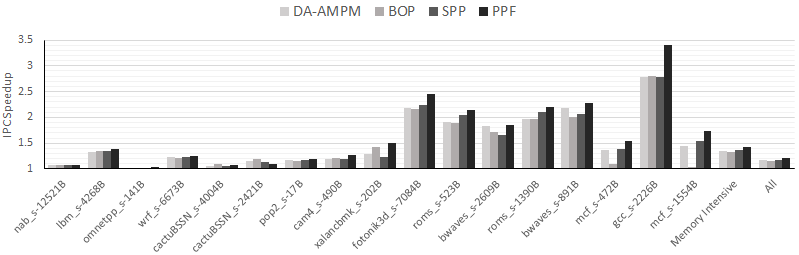
\includegraphics[width=\columnwidth]{SPEC2017}
\caption{SPEC CPU 2017 Single-Core IPC Speedup}
\label{Fig:SPEC2017_1core}
\end{figure}

\section{Results}
\label{Results}

This section discusses the results obtained from running PPF in terms of
prefetch cache coverage and speedup. For the SPEC CPU 2017 benchmarks, first
we present the results for single-threaded workloads then for multi-core
workloads.

\subsection{Single-core Results}
\label{Results-Single}

% djimenez: why is this figure described this way?  it's not OK to just
% highlight noticeable improvement. the benchmarks must be selected by some
% unbiased criteria, e.g. some minimum MPKI under LRU or some minimum speedup
% under a baseline prefetcher that isn't PPF.

Figure~\ref{Fig:SPEC2017_1core} shows the IPC speedup obtained by PPF,
compared to BOP, DA-AMPM and SPP.  In the figure we have depicted selected
traces where PPF shows a noticeable improvement or shows some degradation,
along with the geometric mean improvement on the memory intensive subset of
SPEC CPU 2017, and finally for the complete SPEC CPU 2017 benchmark.  All the
results have been normalized to the baseline of no prefetching.

% djimenez: you've inconsistently italicized and not italicized benchmark
% names. i'll help you out here; i like putting them in a typewriter font so
% i'll do that throughout this section. also, you've inconsistent put and not put
% the number of the benchmark. i'll fix that too.

PPF yields a geometric mean speedup of \textbf{42.8\%} over the baseline. 
This is equivalent to \textbf{7.8\%} over DA-AMPM, \textbf{9.7\%} over BOP 
and \textbf{6.92\%} over SPP.  Out of the 95 simpoints developed for SPEC 
CPU 2017, PPF nearly matches or outperforms most of the prefetchers on 91 
simpoints.  PPF fails to match the improvement offered by BOP only for 
{\tt 607.cactuBSSN\_s} and {\tt 654.roms\_s}.

At its peak, PPF manages a speedup of a factor of over \textbf{3.39x} on the
trace {\tt 602.gcc\_s-2226B}.  This also corresponds to speedup gain of
\textbf{60\%} over the next best prefetcher -- BOP.  In general, benchmarks
{\tt 603.bwaves\_s}, {\tt 605.mcf\_s}, {\tt 623. xalancbmk\_s} and {\tt
649.fotonik3d\_s} benefit the most from PPF, with the speedup over SPP ranging
from \textbf{10\% to 25\%}.

% djimenez: is this geometric mean? if so, say so.
% [EB] Resolved
On the full SPEC CPU 2017 suite, PPF improves the geometric mean IPC of 
the baseline by \textbf{20.9\%}, which is \textbf{3.44\%} better 
than the next best prefetcher -- SPP.
\newline

\begin{figure}[h]
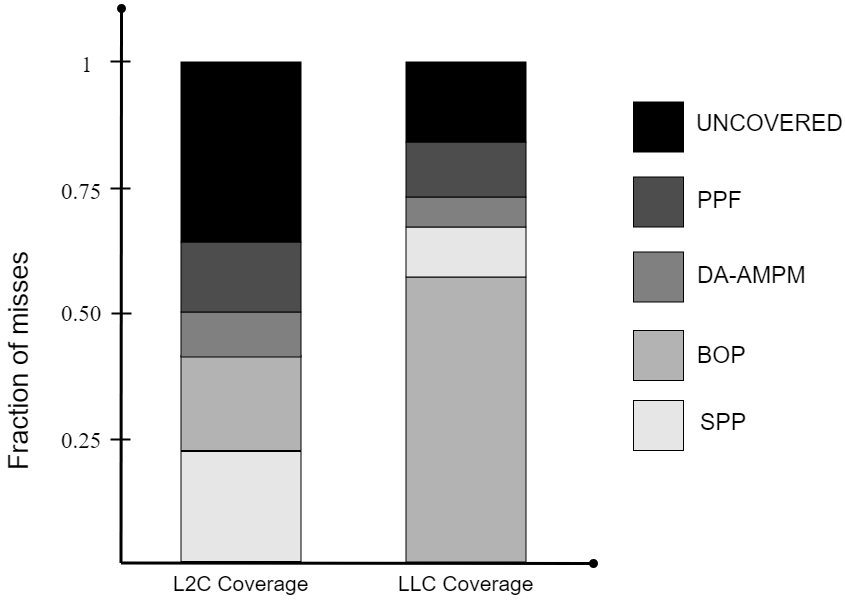
\includegraphics[width=\columnwidth]{Coverage}
\caption{Fraction of Cache Misses Covered}
\label{Fig:Coverage}
\end{figure}

% djimenez: this is a weird way to make a header for a section. use \paragraph or \subsection

\noindent \textbf{COVERAGE}
\newline
Prefetcher coverage is defined as the ratio of the number of misses avoided
through prefetching to the number of misses with no prefetching.

Figure~\ref{Fig:Coverage} shows the fraction of misses in the L2 and LLC
avoided by the various prefetchers.  PPF has the highest coverage of all the
prefetchers simulated. On the SPEC CPU 2017 benchmarks, PPF reduces misses by
\textbf{62.5\%} and \textbf{82.8\%} in the L2 and LLC respectively. For the
same benchmark, the next best prefetcher, DA-AMPM, covers \textbf{48.6\%} and
\textbf{72.8\%} of the misses respectively.

This superior coverage of PPF can be attributed to aggressive re-tuning of the
underlying SPP, enabled by the Perceptron Filter making sure the high coverage
does not lead to increased cache pollution.

\begin{figure*}[ht]
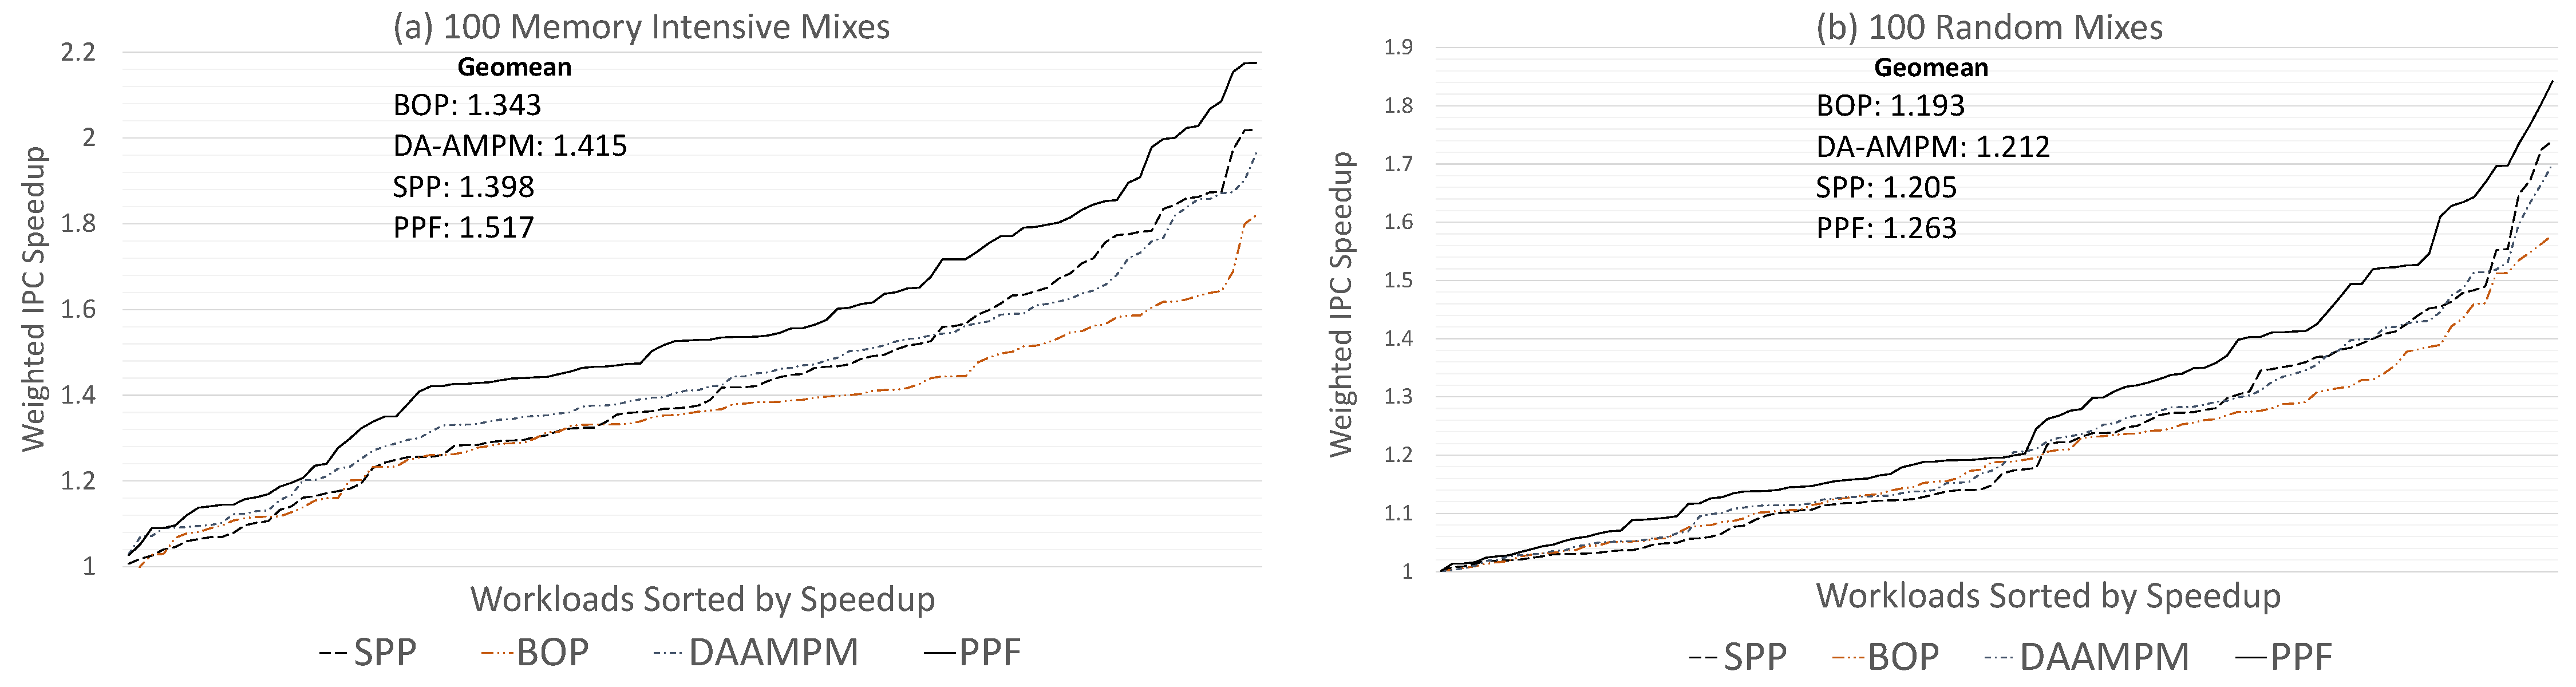
\includegraphics[width=\textwidth]{4Core_SPEC2017}
\caption{Normalized Speedup for 4-core SPEC CPU 2017 Workloads}
\label{Fig:4Core_SPEC2017}
\end{figure*}

\subsection{Multi-core Results}
\label{Results-Multi}
In this section, we demonstrate the improvement achieved by PPF for a mix of
multi-programmed workloads.
\newline

\noindent \textbf{4-CORE ENVIRONMENT}
\newline
Figure~\ref{Fig:4Core_SPEC2017}(a) shows a
comparison of speedups obtained on 4-core mixes of a memory intensive subset
SPEC CPU 2017.  We plot all 4 prefetchers, normalized to the baseline.  The
workloads have been sorted in increasing order of the speedup.  PPF offers a
speedup of \textbf{51.7\%} on these traces, and improvement of \textbf{11.9\%}
over the baseline SPP, \textbf{10.2\%} over the next DA-AMPM, and
\textbf{17.4\%} over BOP.

On a different set of fully random SPEC CPU 2017 4-core mixes, PPF provides an
IPC speedup of \textbf{26.2}\% over the baseline, which is an improvement of
\textbf{5.7}\% over SPP.
\newline

\begin{figure*}[ht]
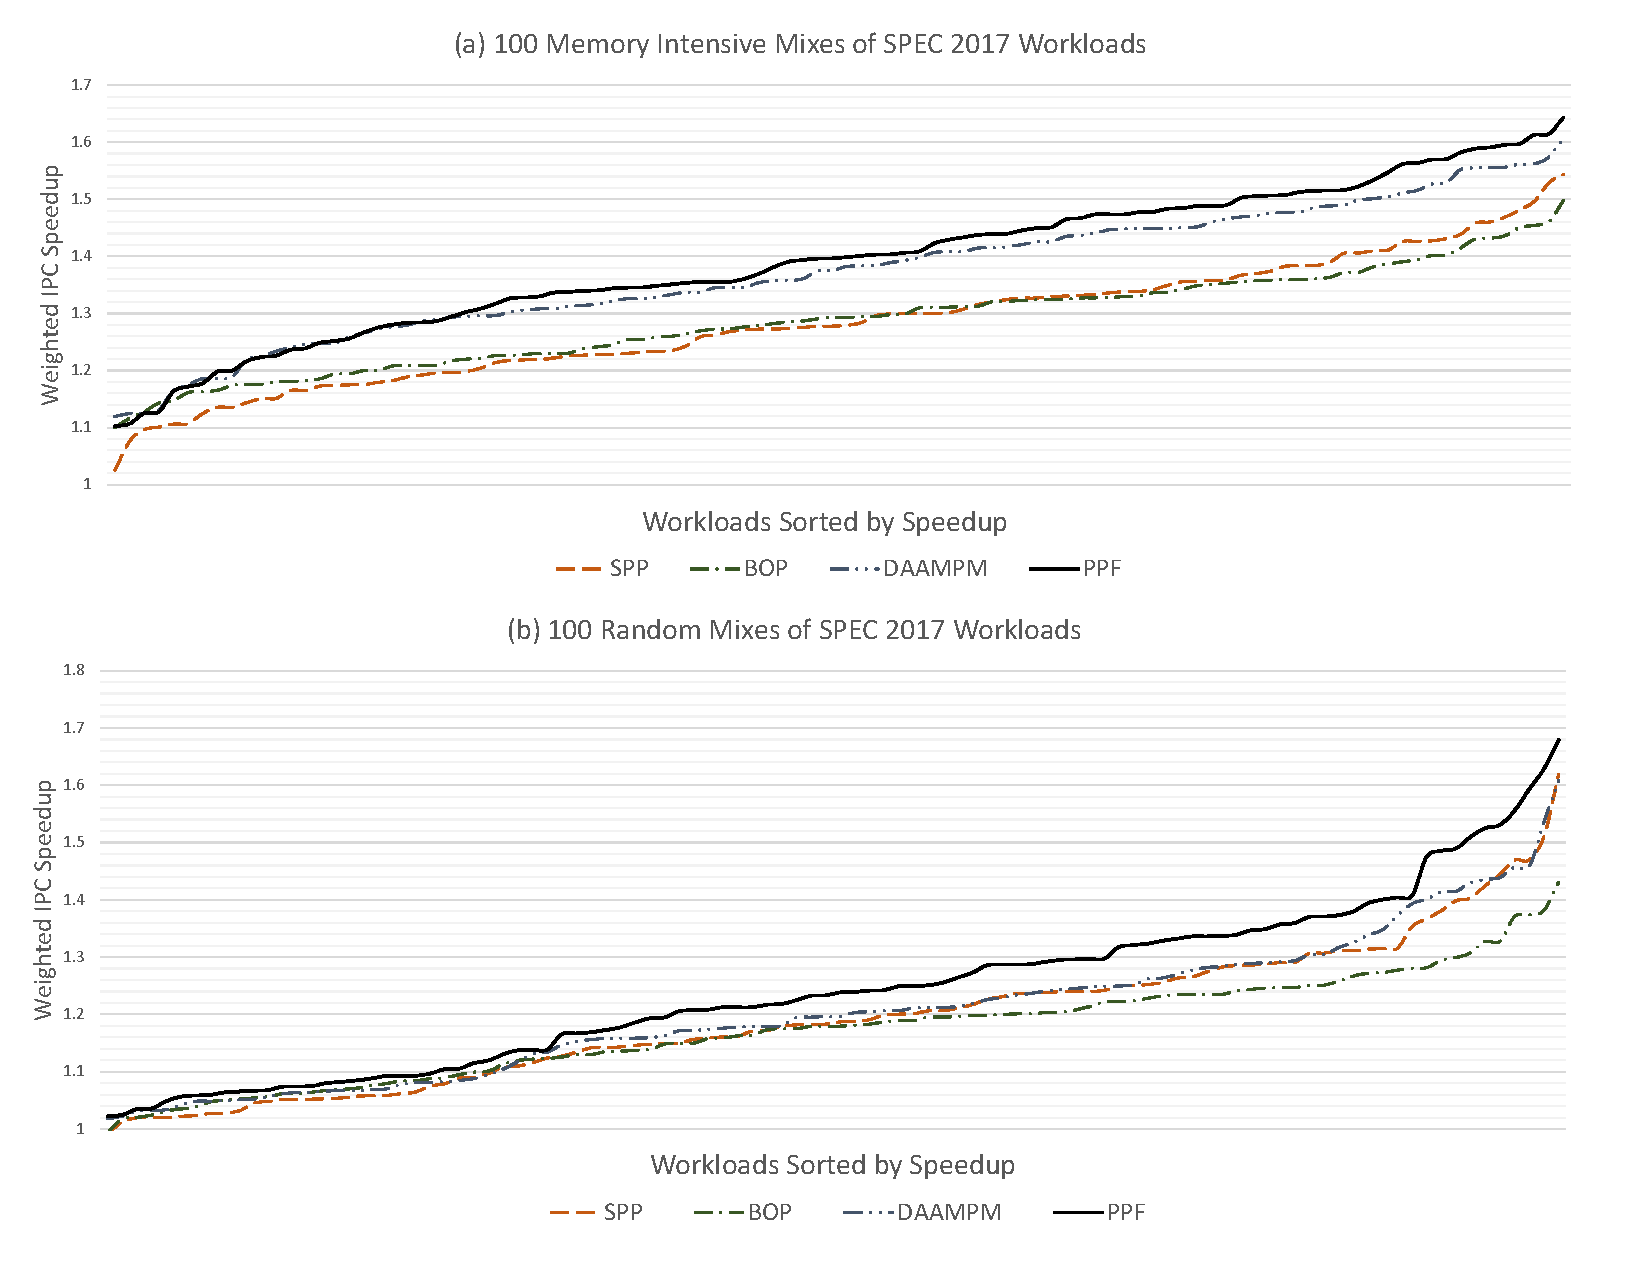
\includegraphics[width=\textwidth]{8Core_SPEC2017}
\caption{Normalized Speedup for 8-core SPEC CPU 2017 Workloads}
\label{Fig:8Core_SPEC2017}
\end{figure*}

\noindent \textbf{8-CORE ENVIRONMENT}
\newline
The sorted comparison of speedups on the memory
intensive 8-core mixes is shown in Figure~\ref{Fig:8Core_SPEC2017}.  PPF
improves baseline performance by \textbf{38.6\%}, an improvement of
\textbf{10.7\%} over SPP.  For a random set of SPEC CPU 2017 mixes, PPF
improves performance by \textbf{23.6\%} over the baseline, corresponding to
\textbf{4.8\%} over SPP.  This increased improvement achieved by PPF over the
base engine SPP in a multi-core environment is expected as PPF has a very
accurate filter, it eliminates useless prefetches before they can cause
pollution in the shared LLC.

BOP offers a better improvement than SPP for the memory intensive mixes. This
superiority can be attributed to BOP's inherent aggressive nature.  DA-AMPM is
also ahead of SPP in both the mixes. Interestingly, in all these cases, PPF
consistently outperforms the best performing prefetcher.

%[EB] How to justify only a small margin over DA-AMPM?

\begin{figure}[ht]
\begin{adjustwidth}{-1cm}{}
  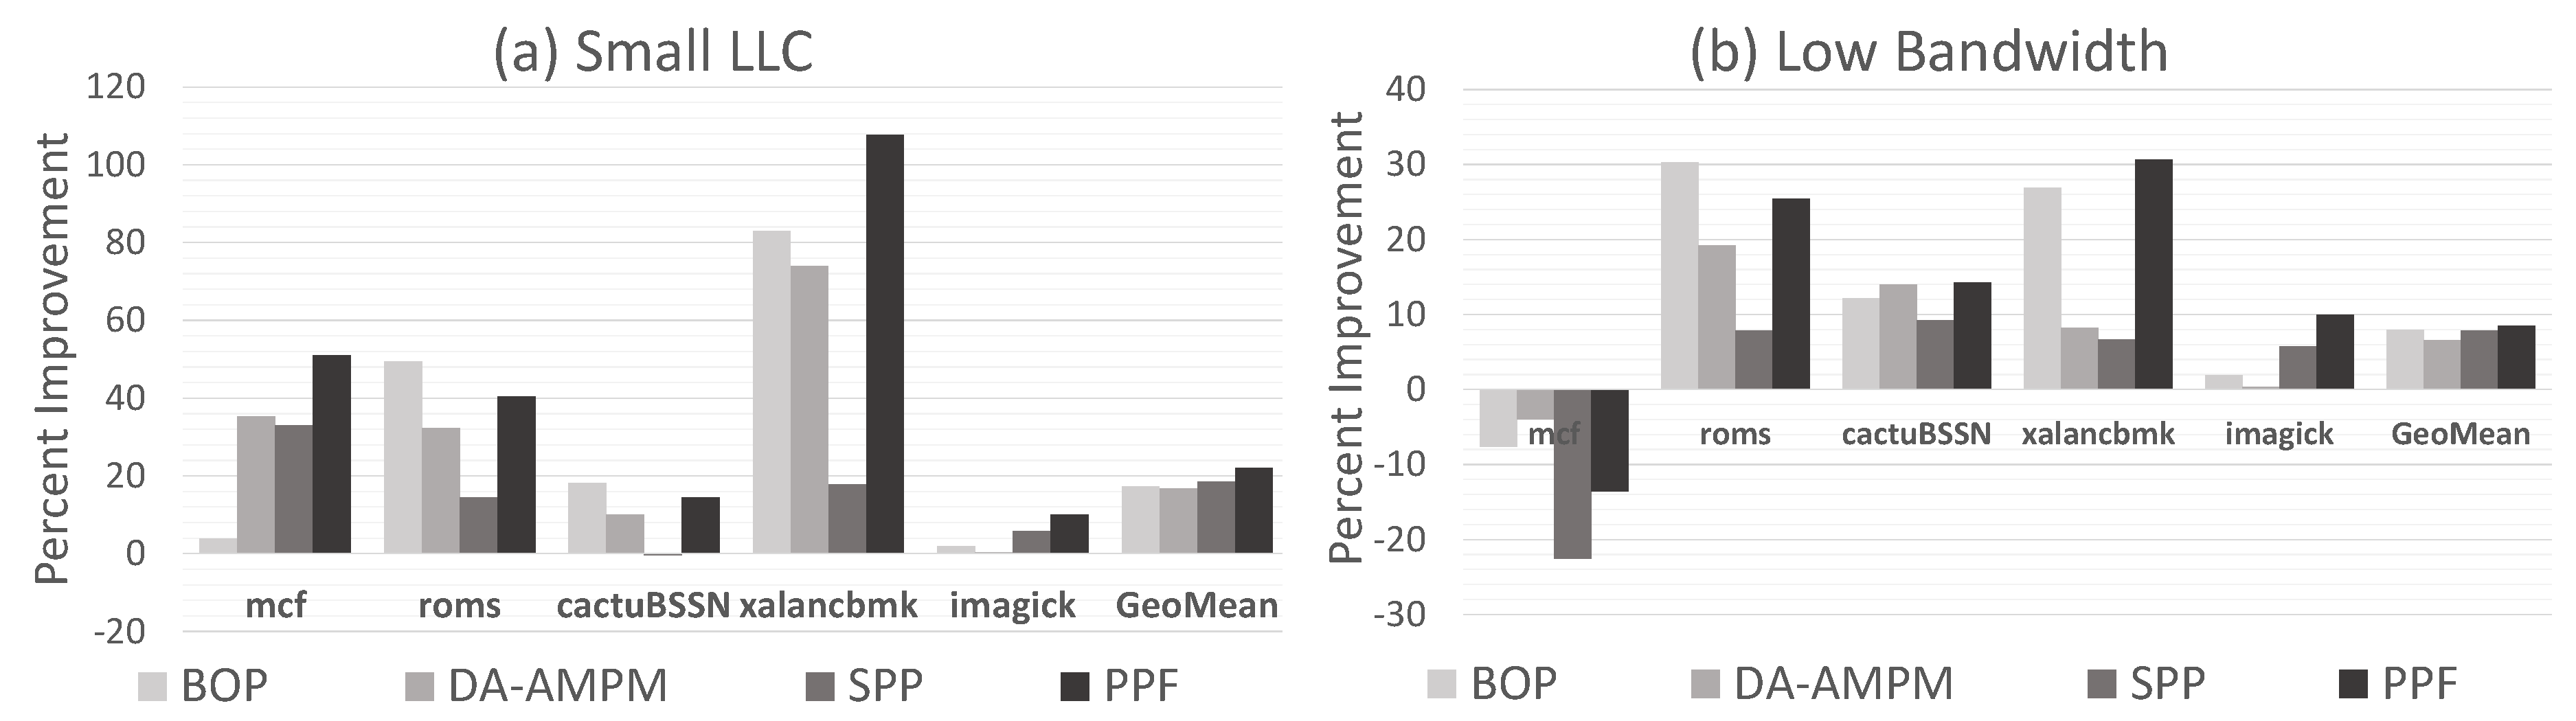
\includegraphics[width=1.2\columnwidth]{AddnConstr}
  \caption{IPC speedup for Small LLC and Low BW}
  \label{Fig:AddnConstr}
\end{adjustwidth}
\end{figure}

\subsection{Additional Memory Constraints}
\label{Results-AdditionalMem}

Figure~\ref{Fig:AddnConstr}(a) and (b) show the performance of PPF in a
reduced LLC and with low bandwidth constraints, respectively. For the sake of
brevity, we have only shown selected traces followed by the overall
performance on the complete benchmark.  Benchmark {\tt 605.mcf\_s} in low
bandwidth conditions is prefetch averse.  In general, any prefetcher yields a
negative speedup on that trace.  On {\tt 654.roms\_s} and {\tt
607.cactuBSSN\_s}, PPF is unable to match the performance achieved by the best
prefetcher. On the other hand, PPF outperforms all the other prefetchers on
{\tt 623.xalancbmk\_s} and {\tt 638.imagick\_s} benchmarks.  Overall, PPF gives
a better improvement under small LLC condition and matches the best
prefetcher, BOP, under low DRAM bandwidth conditions.

\begin{figure}[ht]
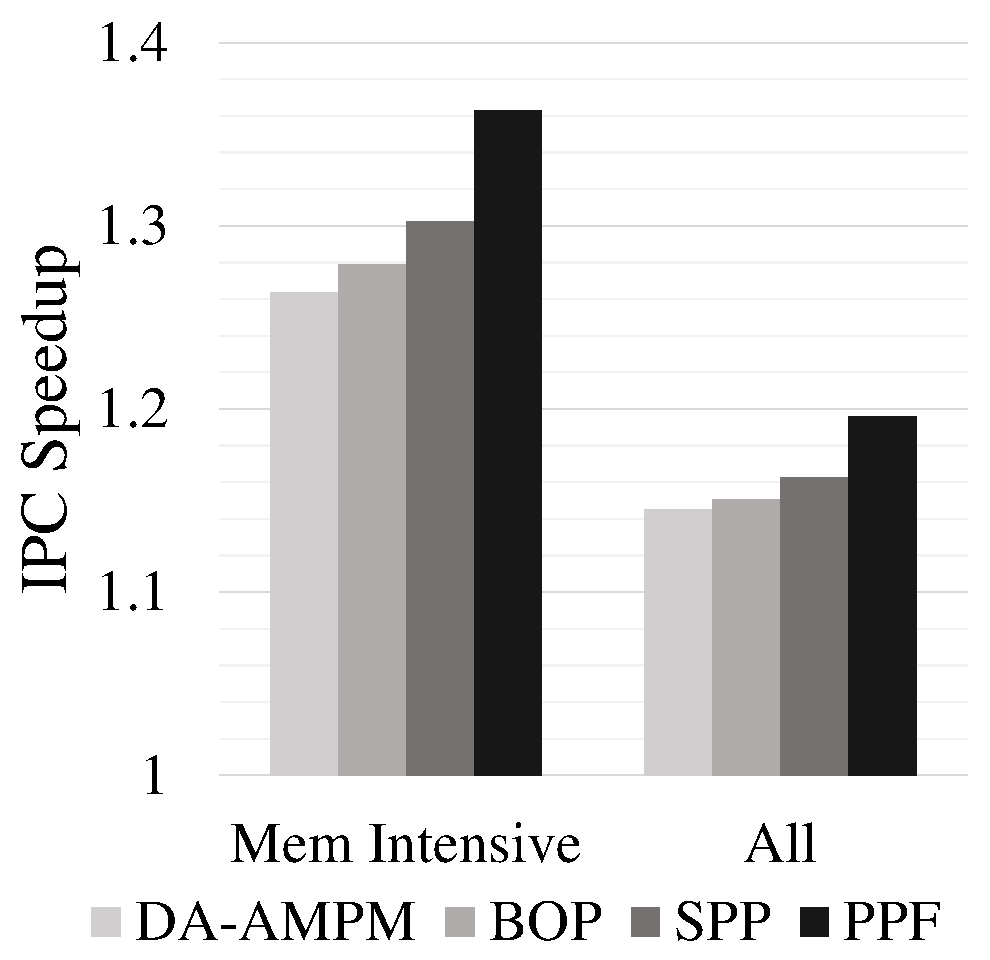
\includegraphics[width=\columnwidth]{SPEC2006}
\caption{SPEC CPU 2006 Single-Core IPC Speedup}
\label{Fig:SPEC2006_1core}
\end{figure}

\begin{figure}[ht]
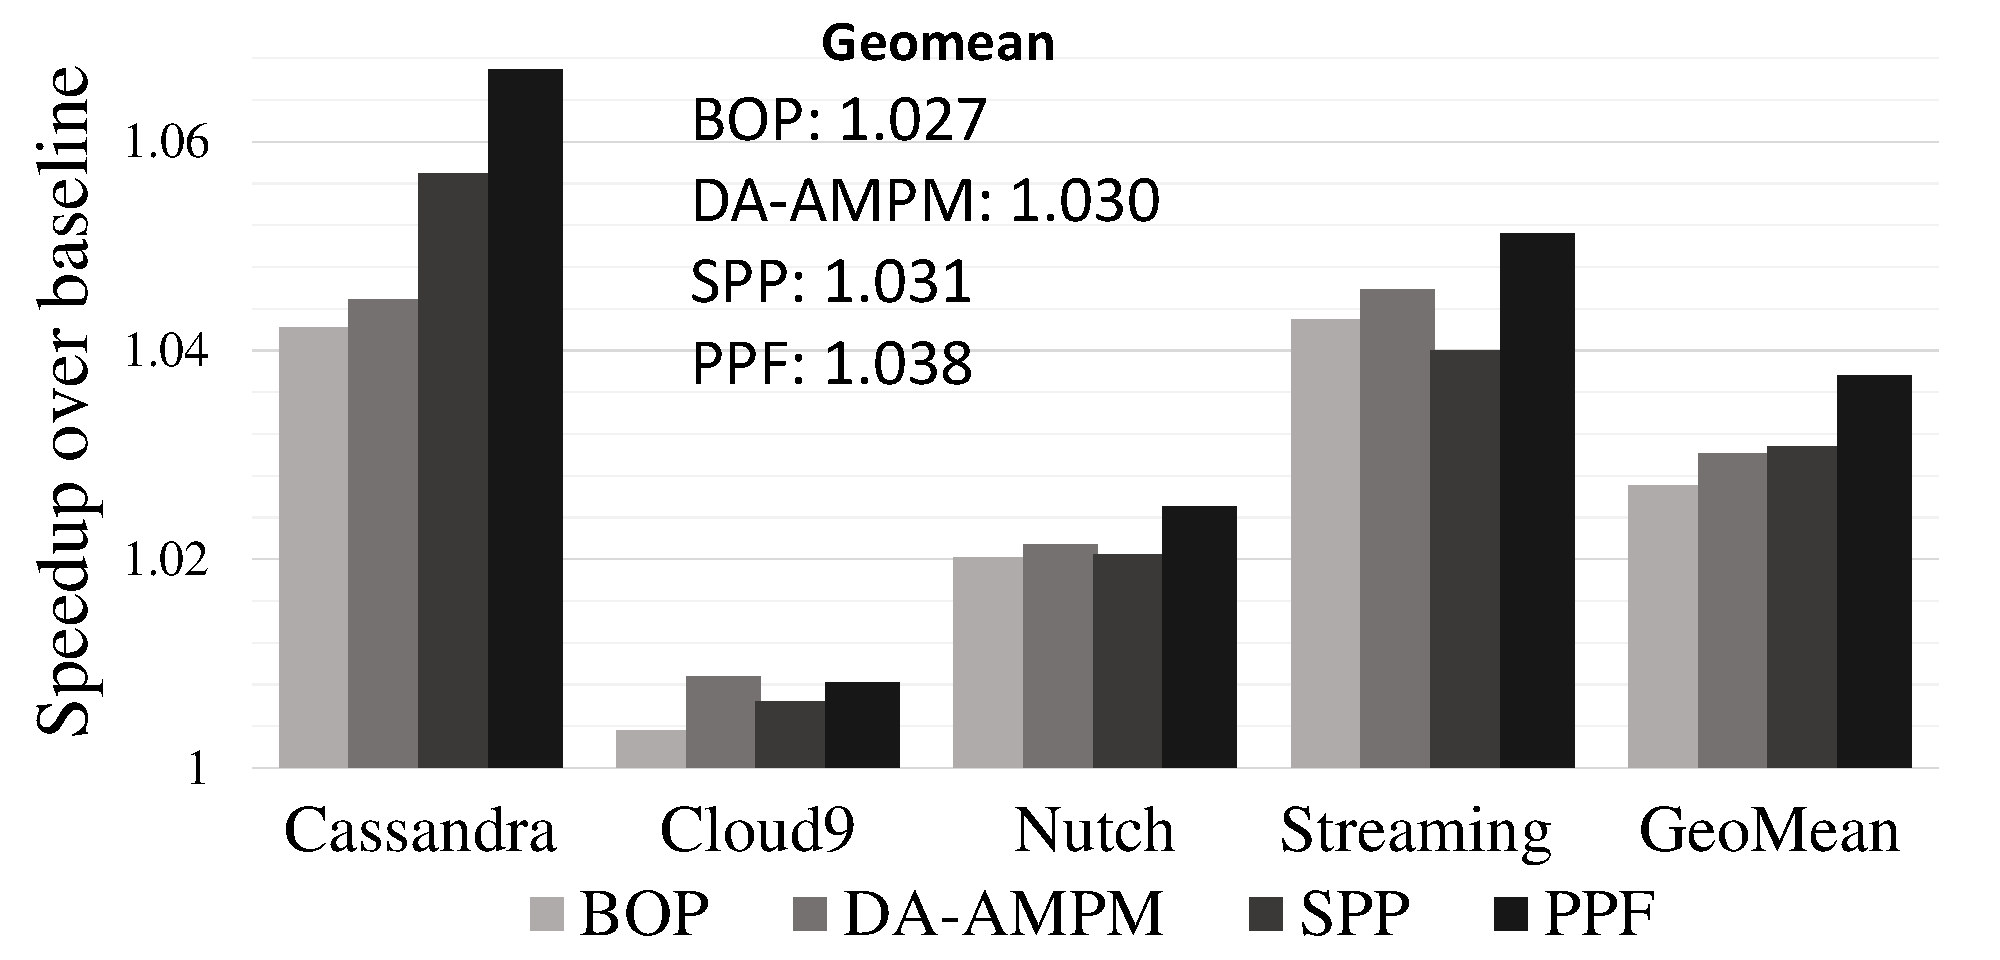
\includegraphics[width=\columnwidth,]{CloudSuite}
\caption{IPC Speedup for Multi-core CloudSuite Workloads}
\label{Fig:CloudSuite}
\end{figure}

\subsection{Cross Validation}
\label{Results-CrossVal}

% djimenez: cite cloudsuite here? do we have a reference?
% [EB]: Resolved. Cited "Clearing the clouds: A study of emerging 
%        scale-out workloads on modern hardware" in methodology

Here we demonstrate the robustness of PPF by testing it on different
benchmarks: SPEC CPU 2006 and CloudSuite.

% djimenez: is the improvement over BOP and DA-AMPM exactly the same 9.86%
% here? that's weird.
% [EB] Resolved. Increased precision of values. But yes, BOP / DA-AMPM 
% have really close numbers for SPEC 2006

Figure~\ref{Fig:SPEC2006_1core} shows the speed-up achieved by BOP, SPP and
PPF on traces from SPEC CPU 2006, along with the overall geometric mean over
the whole suite and over a memory-intensive subset.  PPF provides a speedup of
\textbf{46.1\%} over the baseline on the memory intensive subset of SPEC CPU
2006 benchmark, giving an improvement of \textbf{6.66\%} over SPP and
\textbf{9.88\%} over DA-AMPM and \textbf{9.82} over BOP.  On the whole of 
the SPEC CPU 2006 suite, the speedup is \textbf{22.4\%}, an improvement 
of \textbf{3.34\%} over SPP.

For 4-core memory intensive mixes, PPF improves the baseline by
\textbf{59.2\%}, \textbf{8.7\%} ahead of SPP. For 8-core memory intensive
mixes, the speedup over the baseline is \textbf{47.9\%}, \textbf{11.5\%} ahead
of SPP.

Figure~\ref{Fig:CloudSuite} shows the performance benefit comparison of all
the prefetch schemes on 4 different applications in the CloudSuite benchmark.
In general, these applications are prefetch agnostic. Even so, PPF manages a
\textbf{3.7\%} improvement over no prefetching, putting it ahead of the next
best prefetcher, SPP, which provides a 3.08\% speedup.

We developed PPF to yield good performance on the SPEC CPU 2017 benchmarks.
Nevertheless, the performance is consistently good on other benchmark suites.
We attribute this fact to the inherent adaptability of the perceptron model.
In general, perceptron weights are able to adjust in real-time so as to find
the best possible correlation between the output and the given set of
features.

\section{Conclusion}
\label{Conclusion}
In this paper, we introduced neural network based learning for data
prefetching in the form of PPF.  Perceptron acts an orthogonal
filter to the underlying prefetch engine.  PPF improves
performance by over XX\% over the baseline, which corresponds to YY\%
over the next best performing prefetcher.  
We believe that this is a robust and adaptable technique which can
be used to enhance any existing or upcoming prefetchers.


%%%%%%% -- PAPER CONTENT ENDS -- %%%%%%%%

%%%%%%%%% -- BIB STYLE AND FILE -- %%%%%%%%
\bibliographystyle{ieeetr}
\bibliography{ref}
%%%%%%%%%%%%%%%%%%%%%%%%%%%%%%%%%%%%

\end{document}
